\documentclass[a4paper,french]{paper}
\usepackage{../../_latex_assets/villemejane_iogs_ceti}

%Informations about this document 
%------------------------------------------
\def\module{Conception Electronique pour le Traitement de l'Information}
\def\moduleAbrege{5N-027-SCI / CéTI}
\def\annee{}

\def\titre{Bloc 1 / Capteurs et mise en forme / CORRECTION}
\author{Julien VILLEMEJANE}

\subtitle{Bloc 1}
\institution{LEnsE / Institut d'Optique Graduate School}

\title{\titre}
\usepackage{circuitikz} 

\begin{document} 
%Beginning First Page. 
%------------------------------------------
\enteteThematiqueObligatoire{}

%Beginning Content. 
%------------------------------------------

%%%%%%%%%%%%%%%%%%%
%%%%%%%%%%%%%%%%%%%
%%%%%%%%%%%%%%%%%%%
%%%%%%%%%%%%%%%%%%%
\encadreTDExo{1.1 - Abaisser une tension}{
Proposer un circuit permettant d'abaisser une tension d'un facteur $k$.

$0 < k < 1$ 
}

Pour réduire une tension, il est possible d'utiliser un \textbf{pont diviseur de tension}, basé sur l'utilisation de 2 résistances en série comme proposé dans le schéma suivant.

\medskip

\begin{center}
\begin{circuitikz}
	\draw (1,0) to [short, *-] (3,0)
		to[R=$R_{2}$, -*] (3,2)
		to[R=$R_{1}$, -] (3,4)
		to [short, -*, i<_=$I$] (0,4);
	\draw (3,0) to[short, -o] (4,0);
	\draw (3,2) to[short, -o, i=$I_S$] (4,2);
	
	% fleche
	\draw (0,0.5) edge[->] (0,3.5);
	\node (Ein) at (-1,2.25){$V_E$};

	\draw (0,0) to [short, *-] (1,0)
		node[ground](GND){};
	% fleche
	\draw (3.5,0.3) edge[->, green!40!black] (3.5,1.7); \node[text=green!40!black] (US) at (4,1){$V_S$};
\end{circuitikz}
\end{center}

Pour le calcul, on peut s'intéresser au courant $I$ en écrivant deux lois des mailles différentes :

\begin{enumerate}
	\item $V_E - R_1 \cdot I - R_2 \cdot I = 0$
	\item $V_S - R_2 \cdot I = 0$
\end{enumerate}

Cela suppose que l'on considère que le courant $I_S = 0$.

En combinant les deux, on obtient la relation entre $V_E$ et $V_S$ suivante : $$\boxed{V_S = V_E \cdot \frac{R_2}{R_1 + R_2}}$$

\noindent\hrulefill

\newpage

Si on suppose maintenant que le circuit précédent est chargé par une résistance $R_L$, on obtient alors le montage suivant :

\begin{center}
\begin{circuitikz}
	\draw (1,0) to [short, *-] (3,0)
		to[R=$R_{2}$, -*, i<_=$I_2$] (3,2)
		to[R=$R_{1}$, -] (3,4)
		to [short, -*, i<_=$I$] (0,4);
	\draw (3,0) to[short, -o] (4,0);
	\draw[dashed] (4,0) to[short, -] (5.5,0) 
		to[R=$R_L$, -] (5.5,2)
		to[short, -] (4,2);
	\draw (3,2) to[short, -o, i=$I_S$] (4,2);
	
	% fleche
	\draw (0,0.5) edge[->] (0,3.5);
	\node (Ein) at (-1,2.25){$V_E$};

	\draw (0,0) to [short, *-] (1,0)
		node[ground](GND){};
	% fleche
	\draw (3.5,0.3) edge[->, green!40!black] (3.5,1.7); \node[text=green!40!black] (US) at (4,1){$V_S$};
\end{circuitikz}
\end{center}

Dans ce cas, le courant $I_S$ n'est plus nul.

Le courant $I$ traversant $R_1$ va alors se partager entre $R_2$ et $R_L$. On aura alors la seconde loi des mailles écrites précédemment qui ne sera plus valide.

On peut alors écrire les relations suivantes :
\begin{enumerate}
	\item loi des mailles : $V_E - R_1 \cdot I + V_S$ 
	\item loi des mailles : $V_S - R_L \cdot I_S = 0$  
	\item loi des noeuds : $I = I_S + I_2$ 
	\item loi des mailles : $V_S - R_2 \cdot I_2 = 0$
\end{enumerate}

Après regroupement et simplification, on obtient la relation suivante : $$\boxed{V_S = V_E \cdot \frac{R_{eq}}{R_1 + R_{eq}}}$$  

avec $R_{eq} = \frac{R_2 \cdot R_L}{R_2 + R_L}$ (mise en parallèle de $R_2$ et $R_L$).
 

\newpage
%%%%%%%%%%%%%%%%%%%
%%%%%%%%%%%%%%%%%%%
%%%%%%%%%%%%%%%%%%%
%%%%%%%%%%%%%%%%%%%
\encadreTDExo{1.2 - Élever une tension}{
Proposer un circuit permettant d'élever une tension d'un facteur $k$.

$k > 1$
}

Pour pouvoir élever une tension, il est nécessaire d'\textbf{apporter de l'énergie au montage}. Une solution possible est l'utilisation d'un amplificateur opérationnel (ou amplificateur linéaire intégré - ALI).

On peut par exemple utiliser un montage de type amplificateur non-inverseur dont le schéma est fourni ci-dessous :

\begin{center}
\begin{circuitikz}
	\draw (0,0) node[above]{} to[short, o-, i=$i^+$] ++(1,0)
	node[op amp, noinv input up, anchor=+, fill=blue!10!white](OA){\texttt{AOP1}}
	(OA.-) to[short,-, i<_=$i^-$] ++(0,-1) coordinate(FB)
	to[R=$R_1$, i=$I_1$] ++(0,-2.3) node[ground]{}
	(FB) to[R=$R_2$, *-] (FB -| OA.out) to[short,-, i<_=$I_2$] (OA.out)
	to [short, *-o] ++(1,0) node[above]{};
	\draw (0,-0.3) edge[<-,color={green!40!black}] (0, -4);
	\draw (0,-4.3) to[open,-o] ++(0,0) node[ground](GND){};
	\node[text={green!40!black}] (Ve) at (-0.5,-2.1){$V_E$}; 
	\draw (4.3,-1) edge[<-,color={red}] (4.3, -4);
	\draw (4.3,-4.3) to[open,-o] ++(0,0) node[ground](GND){};
	\node[text={red}] (Vs) at (4.8,-2.7){$V_S$}; 
\end{circuitikz}
\end{center}

Pour pouvoir faire le calcul de la fonction de transfert entre $V_S$ et $V_E$, il est nécessaire de faire \textbf{quelques hypothèses}.

La \textbf{première} vient du fait que les impédances d'entrée de tel amplificateur sont relativement grandes par rapport aux impédances des composants extérieurs ($R_1$ et $R_2$ ici). Les courants d'entrée $i^+$ et $i^-$ peuvent alors être négligés et considérés nuls.

La \textbf{seconde} hypothèse vient ici du fait que l'amplificateur a sa sortie rebouclé avec l'entrée inverseuse (-) par l'intermédiaire d'une résistance. Dans ce cas, on considère que le montage est en \textbf{fonctionnement dit linéaire}. Ainsi, on peut montrer que la différence de potentiel entre $V^+$ et $V^-$ tend vers 0. On peut alors considérer dans ce régime de fonctionnement, que $V^+ = V^-$.

\medskip

Il est alors possible par les lois habituelles de calculer le lien entre $V_S$ et $V_E$.

D'après la première hypothèse, on obtient que $I_1 = I_2$.

D'après la seconde hypothèse, on obtient que $V^- = V_E$.

En calculant le courant $I_1$ par la loi d'Ohm aux bornes de $R_1$, on obtient : $I_1 = \frac{V_E}{R_1}$.

De la même manière, on obtient : $I_2 = \frac{V_S - V_E}{R_2}$.

Après simplification, on obtient alors la fonction de transfert suivante : $$\boxed{V_S = V_E \cdot \frac{R_1 + R_2}{R_1}}$$


\noindent\hrulefill

\textbf{Attention !} Cette loi n'est cependant vraie qu'en basse fréquence et pour des tensions d'entrée faibles.

En effet, les amplificateurs linéaires intégrés sont des composants qui peuvent se modéliser comme un système de type \textbf{passe-bas}.

De plus, ils nécessitent d'être alimentés et lorsque la tension de sortie tend à dépasser la tension d'alimentation, on peut observer un \textbf{phénomène de saturation}.


\newpage
%%%%%%%%%%%%%%%%%%%
%%%%%%%%%%%%%%%%%%%
%%%%%%%%%%%%%%%%%%%
%%%%%%%%%%%%%%%%%%%
\encadreTDExo{1.3 - Limiter une tension}{
Rappeler le fonctionnement d'une diode.

Décrire le fonctionnement du montage suivant :

\begin{center}
\begin{circuitikz}
	\draw (0,0) to[battery2, invert] (0,5) to[short, -] (6,5)
		to[full diode=$D_1$, invert, i<_=$i_1$	] (6,2.5) to[full diode=$D_2$, invert, i<_=$i_2$, *-] (6,0)
		to[short, -*] (3,0) node[ground](GND){} to[short, -] (0,0);
	\draw (3,0) to[sV] (3,2.5) to[R=$R_p$, i=$i_R$] (6,2.5);
	\draw (6,2.5) to[short, -o] (8,2.5);
	\draw (8, 0) to[short, -o] ++(0,0) node[ground](GND){};
	\draw (8,0.3) edge[->,color={red}] (8, 2.2);
	\node[text={red}] (Vs) at (8.5,1.3){$V_S$}; 
	\draw (7,0.3) edge[<-,color={blue}] (7, 2.2);
	\node[text={blue}] (Vd2) at (7.5,1.3){$V_{D2}$}; 
	\draw (7,4.7) edge[->,color={blue}] (7, 2.8);
	\node[text={blue}] (Vd1) at (7.5,3.7){$V_{D1}$}; 
	\draw (2.5,0.3) edge[->,color={green!40!black}] (2.5, 2.2);
	\node[text={green!40!black}] (Ve) at (2,1.3){$V_e$}; 
	\draw (0.7,0.3) edge[->,color={black}] (0.7, 4.7);
	\node[text={black}] (Vcc) at (1.3, 2.5){$V_{CC}$}; 
\end{circuitikz}
\end{center}

}

Loi des mailles du circuit :

\begin{enumerate}
	\item $V_{CC} + V_{D1} + R_p \cdot i_R - V_E = 0$
	\item $-V_{D2} + R_p \cdot i_R - V_e = 0$
	\item $V_{D2} = -V_S$
\end{enumerate}

Les éléments $D_1$ et $D_2$ ont des caractéristiques tension-courant non linéaires.

\begin{center}
\begin{circuitikz}
	\draw (0,0) to[empty diode=$D$, i=$i_d$] (3,0);
	\draw (0,-1) edge[<-,color={blue}] (3, -1);
	\node[text={blue}] (Vd) at (1.5,-1.5){$u_d$}; 
\end{circuitikz}
\end{center}


On peut modéliser les diodes de la manière suivante :
\begin{itemize}
	\item si $u_D > V_F$, $i_d > 0$ et $u_d = V_F$
	\item sinon $i_d = 0$
\end{itemize}

$V_F$ est la tension directe (\textit{forward}) qui est un seuil de conduction dépendant du matériau utilisé. Cette valeur est fournie par le constructeur.

\bigskip

\textbf{Montage}

Comme il y a 2 éléments non linéaires dans le montage à étudier (et comme il y a peu de chance que les deux éléments conduisent ou soient bloquées en même temps), il y a 4 cas à traiter.

Nous allons partir d'une hypothèse sur la conduction des deux éléments et déterminer par la suite dans quelles conditions il est possible d'atteindre cet état.

\bigskip

\textbf{\textit{CAS 1}} $D_1$ et $D_2$ bloquées.

On a $i_1 = i_2 = 0$. Par la loi des noeuds entre les diodes on peut aussi en déduire que $i_r = i_1 + i_2 = 0$.

Ainsi, les lois des mailles 2 et 3 donnent : $V_S = V_E$.

\medskip

Pour être dans ce cas, il est impératif de vérifier les conditions suivantes : $V_{D1} < V_F$ (a) et $V_{D2} < V_F$ (b) (où $V_F$ est la tension seuil de conduction des diodes).

\medskip

\textit{Cas (a)}

$V_{D1} = V_E - V_{CC} - R_p \cdot i_R$ d'après 1

Ainsi $V_{D1} < V_F$ entraîne $V_E - V_{CC} < V_F$ et donc $$\boxed{V_E < V_{CC} + V_F}$$.

\medskip

\textit{Cas (b)}

$V_{D2} = - V_E + R_p \cdot i_R$ d'après 2

Ainsi $V_{D2} < V_F$ entraîne $- V_E < V_F$ et donc $$\boxed{V_E > - V_F}$$.

\medskip

Pour résumé, lorsque $ - V_F < V_e < V_{CC} + V_F $, les deux diodes sont bloquées et $V_S = V_E$.

\bigskip

\textbf{\textit{CAS 2}} $D_1$ bloquée et $D_2$ passante

On a $i_1 = 0$ mais $i_2 \neq 0$. Par la loi des noeuds entre les diodes on peut aussi en déduire que $i_r = -i_2$.

De plus, $V_{D2} = V_F$. D'après 3, on a alors $$\boxed{V_S = -V_F}$$

Cette condition est réalisée lorsque $V_{D2} > V_F$, ce qui entraîne $- V_E > V_F$ et donc $$\boxed{V_E < - V_F}$$.

On peut vérifier que dans cette condition, $D_1$ est bien bloquée.

\bigskip

\textbf{\textit{CAS 3}} $D_1$ passante et $D_2$ bloquée

On a $i_1 \neq 0$ mais $i_2 = 0$. Par la loi des noeuds entre les diodes on peut aussi en déduire que $i_r = i_1$.

De plus, $V_{D1} = V_F$. D'après 1, on a alors $$\boxed{V_S = V_{CC} + V_F}$$

Cette condition est réalisée lorsque $V_{D1} > V_F$, ce qui entraîne $V_E - V_{CC} > V_F$ et donc $$\boxed{V_E > V_{CC} + V_F}$$.

On peut également vérifier que dans cette condition, $D_2$ est bien bloquée.

\bigskip

\textbf{\textit{CAS 4}} $D_1$ et $D_2$ passantes

Ce cas est impossible, d'après les conditions calculées dans le cas 1 (si $V_{CC}$ est strictement positif).

\newpage
%%%%%%%%%%%%%%%%%%%
%%%%%%%%%%%%%%%%%%%
%%%%%%%%%%%%%%%%%%%
%%%%%%%%%%%%%%%%%%%
\encadreTDExo{1.4 - Amplifier un signal}{
Proposer un circuit permettant d'amplifier un signal de $27\operatorname{dB}$, tout en garantissant une bande-passante de $400 \operatorname{kHz}$.

On utilisera des amplificateurs linéaires intégrés de type TL071 (documentation partielle donnée en annexe).
}

On cherche ici à amplifier un signal d'un gain de $27\operatorname{dB}$.

Le gain en décibel $G_{dB}$ est exprimé de la façon suivante en fonction de l'amplification en tension $A_{F}$ : $G_{dB} = 20 \cdot \log(A_F)$.

Il faut dans ce cas une amplification $A_F = 10^{27/20} \approx 22.4\operatorname{V/V}$.

\medskip

Il est possible pour cela d'utiliser une structure de type \textbf{amplificateur non-inverseur} basé sur un \textbf{amplificateur linéaire intégré} ou ALI (de type TL071 comme demandé dans l'énoncé).

Le schéma de base est le suivant : 

\begin{center}
\begin{circuitikz}
	\draw (0,0) node[above]{} to[short, o-, i=$i^+$] ++(1,0)
	node[op amp, noinv input up, anchor=+, fill=blue!10!white](OA){\texttt{AOP1}}
	(OA.-) to[short,-, i<_=$i^-$] ++(0,-1) coordinate(FB)
	to[R=$R_1$, i=$I_1$] ++(0,-2.3) node[ground]{}
	(FB) to[R=$R_2$, *-] (FB -| OA.out) to[short,-, i<_=$I_2$] (OA.out)
	to [short, *-o] ++(1,0) node[above]{};
	\draw (0,-0.3) edge[<-,color={green!40!black}] (0, -4);
	\draw (0,-4.3) to[open,-o] ++(0,0) node[ground](GND){};
	\node[text={green!40!black}] (Ve) at (-0.5,-2.1){$V_E$}; 
	\draw (4.3,-1) edge[<-,color={red}] (4.3, -4);
	\draw (4.3,-4.3) to[open,-o] ++(0,0) node[ground](GND){};
	\node[text={red}] (Vs) at (4.8,-2.7){$V_S$}; 
\end{circuitikz}
\end{center}

D'après les calculs réalisés dans la mission 1.2, on obtient alors la fonction de transfert suivante : $$V_S = V_E \cdot \frac{R_1 + R_2}{R_1}$$

\medskip

Il est alors possible de calculer le rapport $\frac{R_1 + R_2}{R_1}$ en fonction de la valeur d'amplification $A_F$ trouvée.

\textbf{Limites des ALI}

Cependant, si on s'intéresse aux paramètres importants (et limitants) d'un amplificateur linéaire intégré, il existe deux limites importantes :

\begin{itemize}
	\item la \textbf{tension d'alimentation} de l'ALI, qui va impacter la tension maximale admissible en sortie du système. $V_{CC-} < V_S < V_{CC+}$. D'après le \textit{tableau 6.1} de la documentation, on peut noter que l'ALI doit être alimenté de manière symétrique entre -18V et +18V maximum.
	\item le \textbf{produit gain bande-passante} (\textit{GBP} ou \textit{GBW}), qui va limiter la bande-passante du système. En effet, les ALI peuvent être modélisés par un système de type passe-bas dont la fréquence de coupure est liée à l'amplication par la relation suivante : $A_F \cdot BP = B_1$ ($B_1$ correspond à la bande-passante pour un gain unitaire, donc au produit gain bande-passante). $B_1$ est donnée dans le \textit{tableau 6.6} de la documentation et vaut 3~MHz.
\end{itemize}

\medskip

Il est possible de calculer la bande passante théorique du système qu'on cherche à développer autour d'un ALI de type TL071 connaissant $B_1$ et l'amplification recherchée $A_F$.

Ici, on s'aperçoit que la fréquence maximale atteignable dans ces conditions est de $BP = B_1 / A_F = 133\operatorname{kHz}$, donc insuffisante pour le cahier des charges imposé.

L'amplification maximale atteignable pour ce montage afin de respecter une bande passante de $400\operatorname{kHz}$ est de $A_{MAX} = B_1 / BP \approx 7.5\operatorname{V/V}$.

\medskip

\textbf{Mise en cascade}

Pour pouvoir remplir le cahier des charges, il va alors falloir décomposer le système en plusieurs étages.

Ainsi, il est possible de mettre en cascade deux amplificateurs du type précédent. L'amplification totale est alors le produit des deux amplifications. $A_F = A_1 \cdot A_2$. En simplifiant et en prenant $A_1 = A_2$, on en déduit que chaque amplificateur doit avoir une amplification de $A_1 = \sqrt{A_F} \approx 4.7 < A_{MAX}$.

Ainsi, on obtiendra bien un gain de $27\operatorname{dB}$ et une bande passante d'au moins $400\operatorname{kHz}$ (calculée à $BP = B_1 / A_1 = 638\operatorname{kHz}$.

\medskip

\textbf{Choix des valeurs des résistances}

Le calcul précédent impose que pour chaque étage amplificateur : $\frac{R_1 + R_2}{R_1} = 4.7$. Mais il manque une donnée pour pouvoir évaluer les deux inconnues $R_1$ et $R_2$.

Cette seconde "équation" est imposée 
\begin{itemize}
	\item d'une part par une hypothèse émise concernant les courants d'entrée, que l'on a considéré comme nul, et donc par l'impédance d'entrée des ALI, qu'on notera $Z_{ALI}$.
	\item d'autre part par une volonté que notre système consomme le moins possible. En effet, plus les résistances $R_1$ et $R_2$ seront faibles (pour un même potentiel imposé), plus le courant les traversant sera élevé.
\end{itemize} 

D'après le tableau 6.6 de la documentation de l'ALI, on trouve que $Z_{ALI} \approx 10^{12}\operatorname{\Omega}$. Il faut donc que $R_1 + R_2 << Z_{ALI}$ pour pouvoir négliger le courant qui rentrera dans l'ALI par rapport à celui traversant ces résistances.

Pour le second point, il faut tabler sur des courants compris entre $100\operatorname{nA}$ et $1\operatorname{mA}$ traversant les résistances $R_1$ et $R_2$.

Pour des tensions d'environ $10\operatorname{V}$ aux bornes de ces résistances, une résistance de $10\operatorname{k\Omega}$ générera un courant $I = 1\operatorname{mA}$.

Les résistances $R_1$ et $R_2$ doivent donc être choisies autour de $10\operatorname{k\Omega}$.

\newpage
%%%%%%%%%%%%%%%%%%%
%%%%%%%%%%%%%%%%%%%
%%%%%%%%%%%%%%%%%%%
%%%%%%%%%%%%%%%%%%%
\encadreTDExo{1.5 - Additionner des signaux}{
On se propose d'étudier le circuit suivant :
\begin{center}
	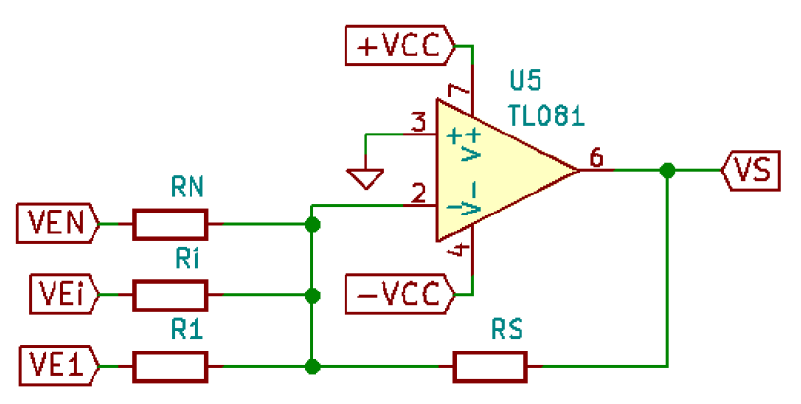
\includegraphics[width=10cm]{images/ali_ampli_somme.png}
\end{center}
}

On fera les \textbf{hypothèses suivantes} :
\begin{itemize}
	\item \textbf{fonctionnement linéaire}, car rebouclage entre la sortie et l'entrée inverseuse par la résistance $R_S$, ainsi $V^+ = V^-$ ;
	\item \textbf{amplificateur parfait}, ainsi $i^+ = i^- = 0$. 
\end{itemize}

\medskip

\textbf{Noeud en $V^-$} $I_S + I_1 + I_i + I_n = 0$

\textit{On supposera les courants positifs ceux venant de l'extérieur du montage.}

\medskip

\textbf{Calcul des courants} par la loi d'Ohm

De plus $V^+ = 0$, ainsi $V^- = 0$.

$I_S = \frac{V_S - V^-}{R_S} = \frac{V_S}{R_S}$

$I_1 = \frac{V_1 - V^-}{R_1} = \frac{V_1}{R_1}$

$I_i = \frac{V_i - V^-}{R_i} = \frac{V_i}{R_i}$

$I_n = \frac{V_N - V^-}{R_N} = \frac{V_N}{R_N}$

\medskip

Après simplification (et généralisation) on obtient alors :

$$V_{S} = -R_S \cdot \sum_{i=1}^{N} \frac{V_i}{R_i} $$


\newpage
%%%%%%%%%%%%%%%%%%%
%%%%%%%%%%%%%%%%%%%
%%%%%%%%%%%%%%%%%%%
%%%%%%%%%%%%%%%%%%%
\encadreTDExo{1.6 - Mettre en forme un capteur de température}{
On se propose d'étudier le circuit suivant :

\begin{center}
	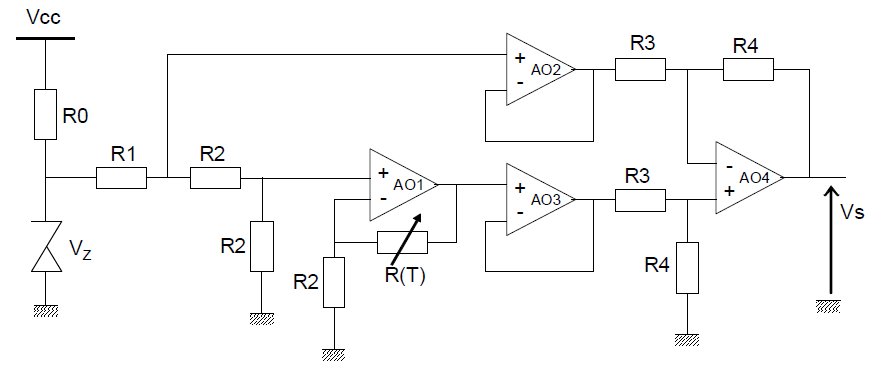
\includegraphics[width=16cm]{images/capteur_conditionnement.png}
\end{center}

La thermistance utilisée est de type PT100. La relation entre sa résistance (en Ohms) et la température (en \degre{}C) est la suivante :
$$R(T) = 100~(1 + 3.908×10^{-3} T - 5.802×10^{-7} T^2)$$

Une partie de la documentation de diodes Zener est fournie en annexe.
}


\textbf{Diode Zener}

On s'intéresse dans un premier temps à la tension en sortie du montage basé sur la diode Zener.

Une diode Zener est un composant non linéaire, qui possède deux zones "passantes", contrairement à des diodes de signal plus classiques qui ne possède qu'une zone "passante" pour des tensions positives (voir caractéristique ci-dessous).

\begin{center}
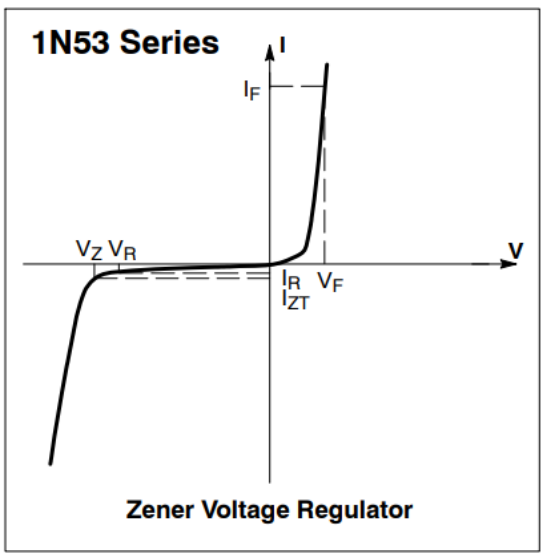
\includegraphics[width=6cm]{images/zener_carac.png}
\end{center}

\begin{center}
\begin{circuitikz}
	\draw (0,0) to[empty Zener diode=$D_Z$, i=$i_d$] (3,0);
	\draw (0,-1) edge[<-,color={blue}] (3, -1);
	\node[text={blue}] (Vd) at (1.5,-1.5){$u_d$}; 
\end{circuitikz}
\end{center}

Il existe alors deux limites de conduction :
\begin{itemize}
	\item si $u_d > V_F$, alors $i_d > 0$ (sens direct)
	\item si $u_d < - V_Z$, alors $i_d < 0$ (sens Zener)
	\item sinon $i_d = 0$
\end{itemize}

\textbf{Montage Zener}

\begin{center}
\begin{circuitikz}
	\draw (0,0) node[ground]{} 
		to[empty Zener diode=$D_Z$, i=$i_d$, -*] (0,2.5)
		to[R=$R_0$, i<_=$i_0$] (0,5)
		to[short, -] (-2,5)
		to[battery2] (-2,0)
		to[short,-*] (0,0);
	\draw[dashed] (0,2.5) to[short, -o, i=$i_s$] (2,2.5);
	\draw[dashed] (0,0) to[short, -o] (2,0);
	\draw (2,0.3) edge[<-,color={blue}] (2, 2.2);
	\node[text={blue}] (Vd) at (2.5,1.2){$u_d$};
	\draw (3,0.3) edge[->,color={red}] (3, 2.2);
	\node[text={red}] (Vs) at (3.5,1.2){$V_S$};
	\draw (-1.5,0.3) edge[->,color={black}] (-1.5, 4.7);
	\node[text={black}] (Vcc) at (-1,2.5){$V_{CC}$};
\end{circuitikz}
\end{center}

Loi des mailles : $V_{CC} - R_0 \cdot i_0 + u_d = 0$

Ainsi : $u_d = R_0 \cdot i_0 - V_{CC}$

\textbf{\textit{Cas 1 (sens direct)}}

Pour que la diode soit passante dans le sens direct, il faut que $u_d > V_F$, c'est à dire que $R_0 \cdot i_0 - V_{CC} > V_F$.

On obtient alors, à la limite de conduction (lorsque $i_0 = 0^+$), la condition que $V_{CC} < -V_F$.

Par principe $V_{CC}$ sera positif. Ce cas est donc impossible.


\textbf{\textit{Cas 2 (sens Zener)}}

Pour que la diode soit passante dans le sens Zener, il faut que $u_d < -V_Z$, c'est à dire que $R_0 \cdot i_0 - V_{CC} < -V_Z$.

On obtient alors, à la limite de conduction (lorsque $i_0 = 0^+$), la condition que $V_{CC} > V_Z$. Dans cette condition, $u_d = -V_Z$ et donc $V_S = -u_d = V_Z$ !

Dans cette condition, la tension $V_S$ de ce montage est (quasi)constante et égale à la tension Zener.

On obtient un \textbf{régulateur de tension}.


\textbf{Etude du montage}

Pour étudier ce circuit, on commence par \textbf{décomposer en blocs} plus facilement calculables, en partant du signal de sortie.

De manière générale, chaque amplificateur linéaire (ALI) correspond à un montage particulier. Il peut donc être intéressant d'identifier les montages associés à chaque ALI.

Ici, on peut décomposer de cette façon : 
\begin{itemize}
	\item Autour de l'AO4 : amplificateur différentiel 
	\item Autour des AO2 et AO3 : suiveur / découplage
	\item Autour de l'AO1 : montage linéaire de type amplificateur / tension de sortie dépendante de la température
	\item Autour de la diode Zener : tension de référence	
\end{itemize}


\textbf{AO1} 

Hypothèse classique : fonctionnement linéaire ($V^+ = V^-$) et ALI parfait ($i^+ = i^- = 0$).

$V+ = V_Z \cdot R_2 / (R_1 + 2 R_2)$ et $V- = V_1 \cdot R_2 / (R_2 + R(T))$, alors : 

$$V_1 = V_Z \cdot \frac{R_2}{R_1 + 2 R_2} \cdot \frac{R_2 + R(T)}{R_2} = V_Z \cdot \frac{R_2 + R(T)}{R_1 + 2 R_2}$$

\textbf{AO2} : suiveur / diviseur de tension

$$V_2 =  V_Z \cdot \frac{2 \cdot R_2 + R(T)}{R_1 + 2 R_2}$$

\textbf{AO3} : suiveur

$$V_3 = V_1$$

\textbf{AO4} 

$V- = (V_S/R_4 + V_2/R_3) / (1/R_3 + 1/R_4)$ (Millmann)

$V+ = V_3 \cdot R_4 / (R_3 + R_4)$

On a alors : 

$$V_S = (V_3 - V_2) \cdot \frac{R_4}{R_3}$$


\textbf{Montage complet}

$$V_S = V_Z \cdot \frac{R_4}{R_3} \cdot \frac{R(T) - R_2}{R_1 + 2 R_2}$$

$$V_S = V_Z \cdot \frac{R_4}{R_3} \cdot \frac{R_2}{R_1 + 2 R_2} \cdot (\frac{R(T)}{R_2} - 1)$$


Lorsque $T < 0$, $R(T) < R_2$ et donc $V_S < 0$. Alimentation symétrique indispensable.


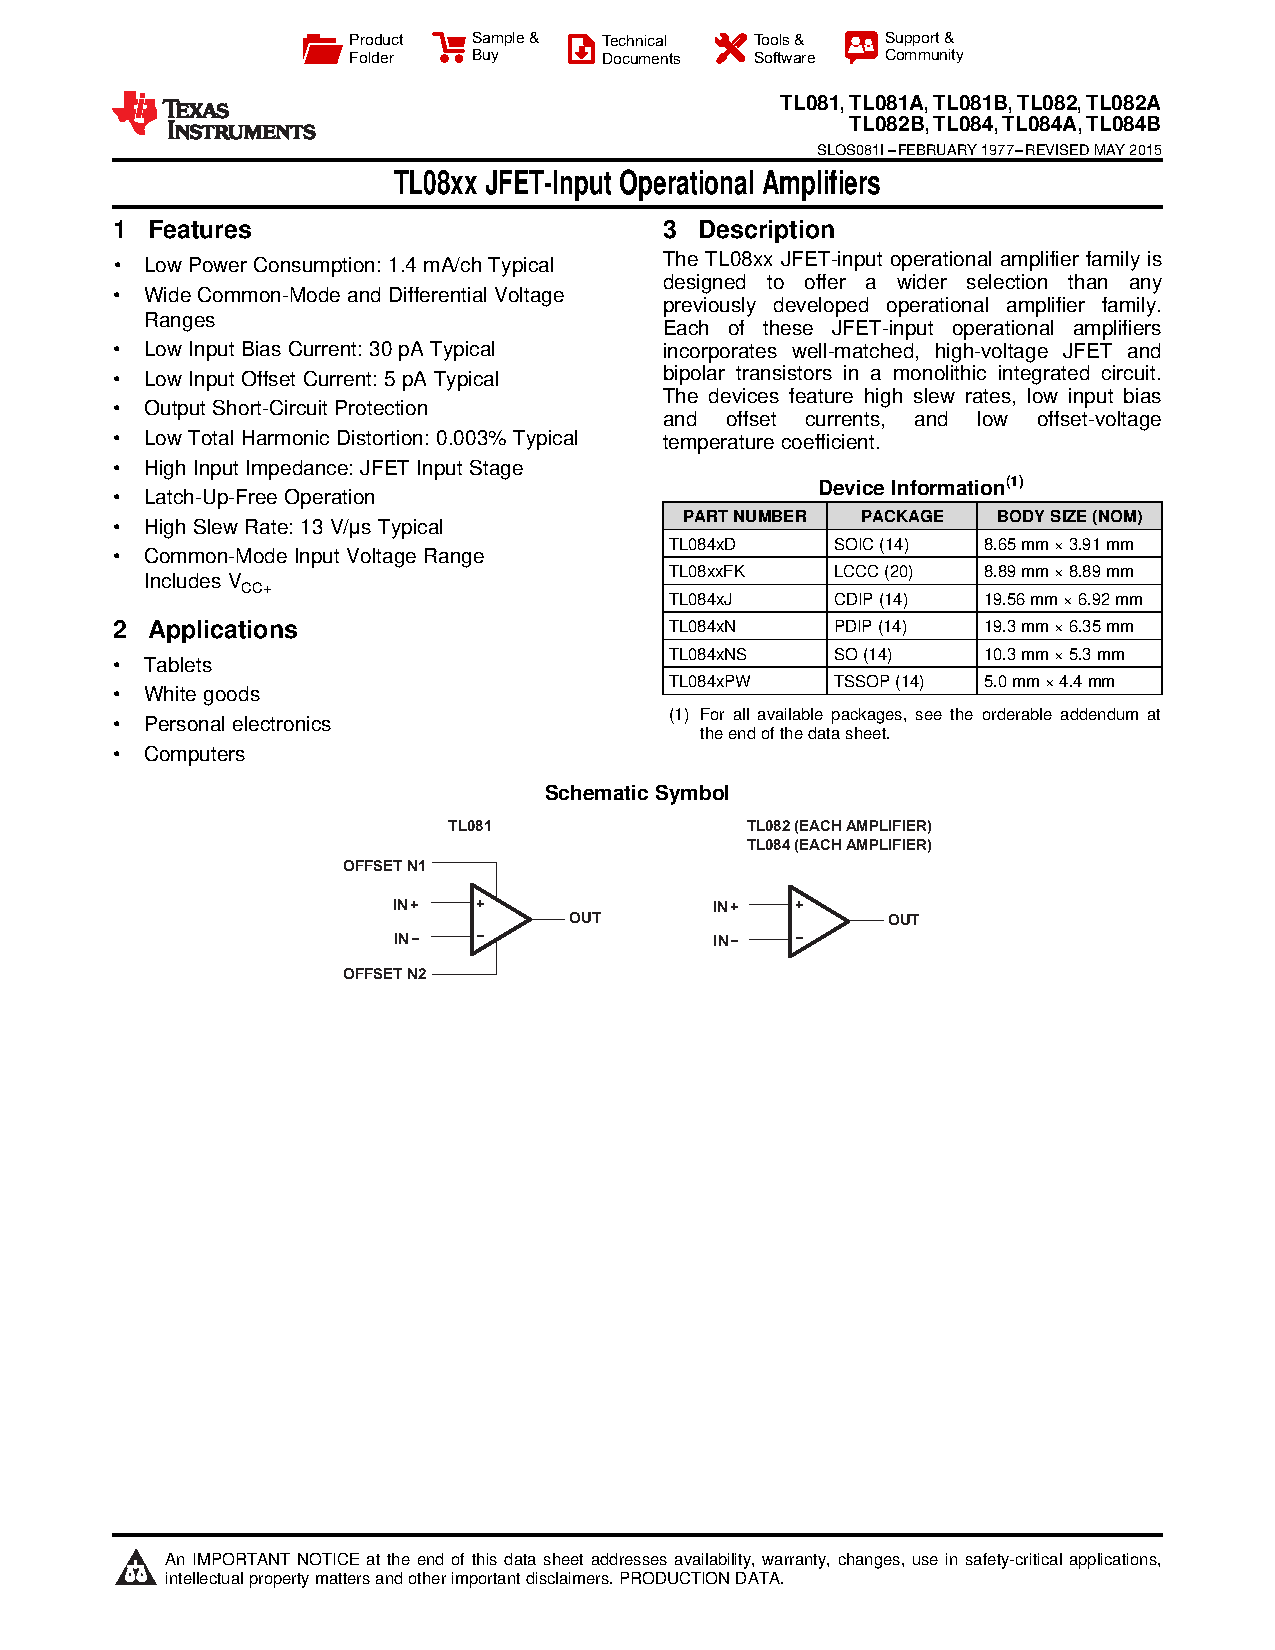
\includepdf[pages=-]{doc/doc_TL071_1p.pdf}
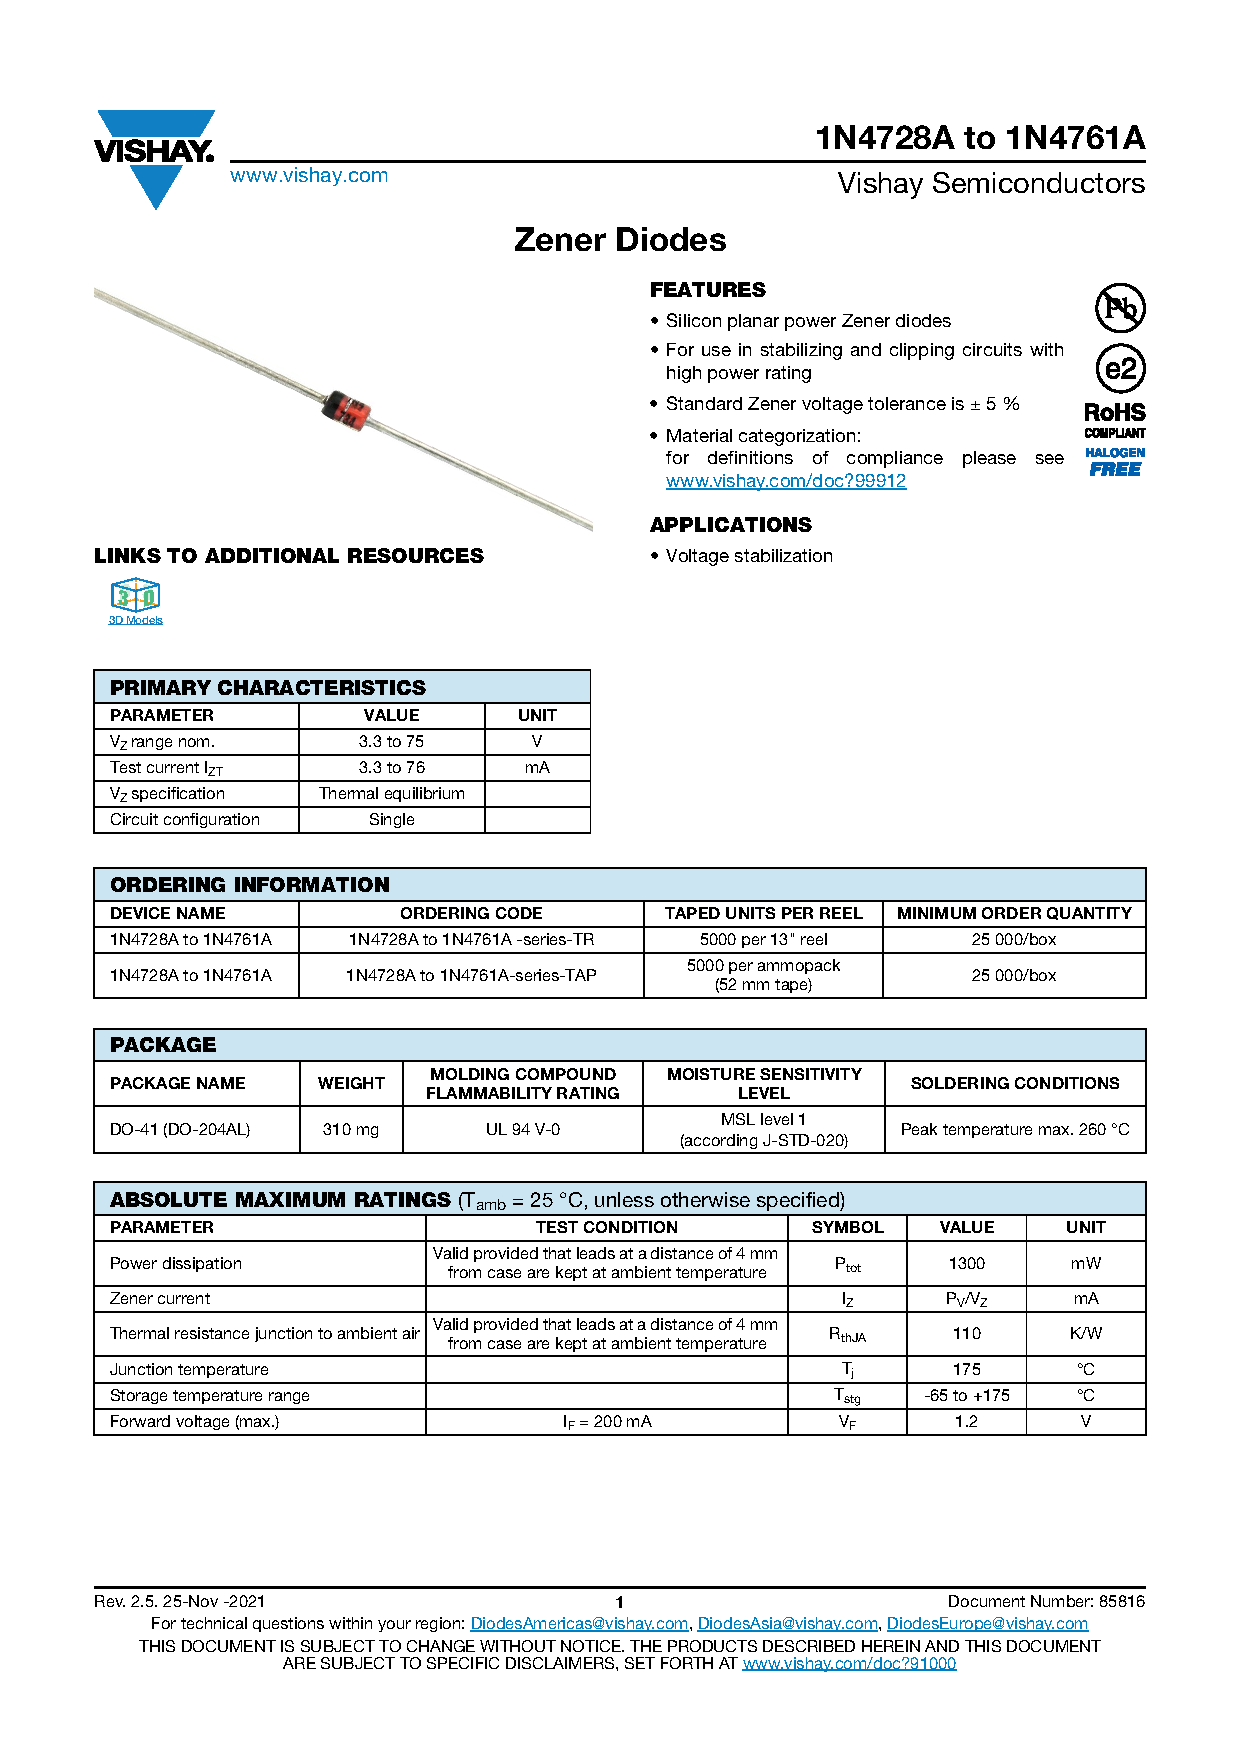
\includepdf[pages=1-2]{doc/1n4728a.pdf}

\end {document}